\documentclass{standalone}
\usepackage{tikz}
\usetikzlibrary{shapes.geometric}

\begin{document}
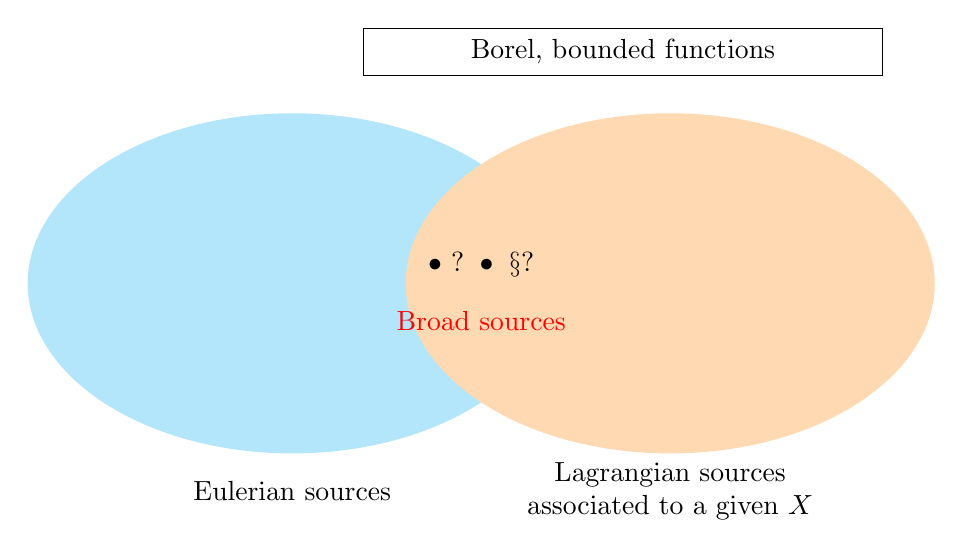
\begin{tikzpicture}[scale=1.2]

% Title box
\draw (0.25,2.2) rectangle (5.75,2.7);
\node at (3,2.45) {Borel, bounded functions};

% Left ellipse (light blue fill)
\fill[cyan!30] (-0.5,0) ellipse (2.8cm and 1.8cm);

% Right ellipse (light orange fill)
\fill[orange!30] (3.5,0) ellipse (2.8cm and 1.8cm);

% Intersection labels
\node at (1.5,0.2) {$\bullet\ ? \ \bullet\ \S?$};
\node at (1.5,-0.4) [red] {Broad sources};

% Bottom labels
\node at (-0.5,-2.2) {Eulerian sources};
\node[align=center] at (3.5,-2.2) {Lagrangian sources\\associated to a given $X$};

\end{tikzpicture}
\end{document}